\documentclass[aps,tightenlines,16pt]{ctexart}

\usepackage{slashed}
\usepackage{amsmath,amsfonts,amssymb}
% \usepackage{bm}  %黑体希腊字母
\usepackage{bbm} %空心字母数字
\usepackage{ctex}
\usepackage{float}
%\usepackage[dvips]{graphicx}
\usepackage[english]{babel}
\allowdisplaybreaks[4]  %公式环境换行
\numberwithin{equation}{section}
\usepackage{slashed} %费曼slashed
\usepackage[left=2cm,right=2cm,top=2.54cm,bottom=2.54cm]{geometry}
%\usepackage[dvipdfm,pdfstartview=FitH]{hyperref}
%\usepackage{cancel}
%\usepackage{forest}
%\usepackage{leftidx}  %设置上下标
\usepackage{cite}
\usepackage[justification=centering]{caption}
\usepackage{graphicx, subfigure}
\usepackage{indentfirst}  %段落首行缩进
\usepackage{hyperref}  %设定引用公式跳转链接
\usepackage{color}  %设置字体颜色
\usepackage{tikz,pgf}
% \usepackage{tikz-3dplot}
\usepackage{tikz-feynman} 
% \tikzfeynmanset{compat=1.1.0}
% \tikzfeynmanset{
%         every vertex={dot},
%         every particle={blue},
%         every blob={draw=green!40!black,pattern color=
%         green!40!black},
%         }
\usepackage{braket}
%\usepackage{txfonts}  %平行符号
%\usepackage{fancyhdr}  %左偶右奇
\usepackage{multirow}
\usepackage{booktabs}
\usepackage{cancel}   
\usepackage{threeparttable}  
\usepackage{diagbox}
\usepackage{extpfeil}  %等号上加文字
\usepackage{extarrows}

\usetikzlibrary{calc}
%\usetikzlibrary{arrows.meta}
\usetikzlibrary{intersections}
\usetikzlibrary{trees}
\usetikzlibrary{decorations.pathmorphing}
\usetikzlibrary{decorations.markings}
\usetikzlibrary{patterns}
\tikzset{
   global scale/.style={
      scale=#1,
      every node/.append style={scale=#1}},
   photon/.style={decorate, decoration={snake}, draw=red},
   nucleon/.style={draw=black, postaction={decorate},
      decoration={markings,mark=at position .55 with{\arrow[draw=black]{>}}}},
   pion/.style={draw=blue, postaction={decorate},
      decoration={markings,mark=at position .55 with{\arrow[draw=blue]{}}}},
    }


% \newcommand{\bl}{\boldsymbol{l}}
% \newcommand{\bk}{\boldsymbol{k}}
% \newcommand{\bp}{\boldsymbol{p}}
% \newcommand{\bP}{\boldsymbol{P}}
% \newcommand{\bq}{\boldsymbol{q}}
% \newcommand{\bA}{\boldsymbol{A}}
% \newcommand{\bM}{\boldsymbol{M}}
% \newcommand{\bV}{\boldsymbol{V}}
% \newcommand{\ba}{\boldsymbol{a}}
% \newcommand{\bb}{\boldsymbol{b}}
% \newcommand{\bx}{\boldsymbol{x}}
% \newcommand{\bep}{\boldsymbol{\epsilon}}
% \newcommand{\bsi}{\boldsymbol{\sigma}}
% \newcommand{\bL}{\boldsymbol{L}}
% \newcommand{\bJ}{\boldsymbol{J}}
% \newcommand{\br}{\boldsymbol{r}}
% \newcommand{\bs}{\boldsymbol{s}}
% \newcommand{\bS}{\boldsymbol{S}}
% \newcommand{\bi}{\boldsymbol{i}}
% \newcommand{\bI}{\boldsymbol{I}}
% \newcommand{\bB}{\boldsymbol{B}}  
\newcommand{\sP}{\slashed{P}} 
\newcommand{\spp}{\slashed{p}} 
\newcommand{\sk}{\slashed{k}} 
\newcommand{\sq}{\slashed{q}}
\newcommand{\sD}{\slashed{D}} 
\newcommand{\sA}{\slashed{A}}
\newcommand{\spa}{\slashed{\partial}}
% \newcommand{\sep}{\slashed{\epsilon}} 
% \newcommand{\spar}{\slashed{\partial}} 
% \newcommand{\Pmu}{P^\mu} 
% \newcommand{\pmu}{p^\mu} 
% \newcommand{\kmu}{k^\mu} 
% \newcommand{\qmu}{q^\mu}
% \newcommand{\gmu}{\gamma^\mu}
% \newcommand{\bpi}{\boldsymbol{\pi}}
% \newcommand{\btau}{\boldsymbol{\tau}}
% \newcommand{\brho}{\boldsymbol{\rho}}
\newcommand{\md}{\mathrm{d}}
% \newcommand{\mB}{\mathbf{B}}
\newcommand{\mD}{\mathcal{D}}
\newcommand{\mO}{\mathcal{O}}
\newcommand{\mL}{\mathcal{L}}
% \newcommand{\bm}[1]{\mbox{\boldmath{$#1$}}}

\allowdisplaybreaks


\begin{document}\large
     \title{axions}
     
\renewcommand{\today}{\number\year 年 \number\month 月 \number\day 日}
 \author{王旭}
 \maketitle
 %\newpage
 \setlength{\parindent}{2em}  %首行缩进两个中文字符
 \hypersetup{hypertex=true,
            colorlinks=true,
            linkcolor=blue,
            anchorcolor=blue,
            citecolor=blue}  %设定引用公式跳转链接
 \renewcommand\thesubsection{\arabic {subsection}}
 \renewcommand\contentsname{目录}
\tableofcontents
\newpage 

%! TEX root = ./axions.tex
\section{简介}
首先,什么是轴子?
\begin{enumerate}
   \item 轴子场是周期性场,即$a(x)=a(x)+2\pi f_a$,其中$f_a$是轴子的衰变常数。
   \item 轴子场和pseudo shift-symmetry相关联。
   \item 轴子场是$U(1)_{PQ}$对称性自发破缺产生的pseudo Goldstone Boson。
   \item 轴子场是用来解决强CP问题(强相互作用中CP不破坏)而被提出。
\end{enumerate}
\subsection{EFT以及QCD反常}
考虑一个复场$\phi$,具有$U(1)$对称性$\phi:\stackrel{U(1)}{\longmapsto} e^{i\alpha}\phi$,假设$Q=1$。则拉氏量的写法为
\begin{equation}
   \mL = \partial_{\mu} \phi^{*} \partial^{\mu} \phi-V(\phi^*\phi),\ V=\lambda(\phi^*\phi-\frac{f^2}{2})^2.
\end{equation}
令$x=\phi^*\phi$,则
\begin{equation*}
   0=\frac{\partial V}{\partial x}=2\lambda(x-\frac{f^2}{2})\Rightarrow \langle \phi^*\phi\rangle = \frac{f^2}{2}.
\end{equation*}
%! TEX root = ../axions.tex
\begin{figure}[h]
    \centering
    \begin{tikzpicture}
        [x={(0.8cm,0cm)},z={(0cm,0.1cm)},y={(-0.4cm,-0.7cm)}]
        \draw[->,thick,black!70] (0,0,0) -- (4,0,0) node[right] {Im$\phi$}; % 虚轴
        \draw[->,thick,black!70] (0,0,0) -- (0,4,0) node[below right] {Re$\phi$}; % 实轴
        \draw[->,thick,black!70,scale=0.1] (0,0,0) -- (0,0,600) node[above] {V}; % 势能 
        
        % ellipse
            \def \rx{1.5}
            \def \ry{1}
            \def \z{0}
            \draw[rotate around={-12:(0,0,0)},dashed]  ellipse({\rx} and {\ry});
            \def \nx{2.88}
            \def \ny{1.44}
            \def \tz{41}
            \def \tx{-0.6}
            \draw[rotate around={-7:(0,0,0)},dashed] (\tx,0,\tz
            ) ellipse({\nx} and {\ny});
        % function
        \draw[domain=-3:3,samples=200,smooth]
        plot(\x,0,{(\x*\x-2.5)^2});

        \end{tikzpicture}
\end{figure}

重新参数化$\phi$为$\phi=\frac{f+\rho}{\sqrt{2}}e^{ia/f}$。此时$U(1)$变换为
\begin{align}
   \begin{aligned}
      \phi = \frac{f+\rho}{\sqrt{2}}e^{ia/f}&\rightarrow e^{i\alpha}\phi\\
      a &\rightarrow a + \alpha f.
   \end{aligned}
\end{align}
场$a$的对称性变为shift-symmetry。

将拉氏量用新的参数描述
\begin{equation}
   \mL = \frac{1}{2}\partial_{\mu}\rho \partial^{\mu}\rho + \frac{1}{2}(1+\frac{\rho}{f})^2\partial_{\mu}a\partial^{\mu}a-\frac{1}{2}m_{\rho}^2\rho^2-\frac{m_{\rho}^2}{2f}\rho^3-\frac{m_{\rho}^2}{8f^2}\rho^4,
\end{equation}
其中$m_{\rho}^2=2\lambda f^2$。
\textcolor{blue}{$E<<f,f\ge 10^3GeV$}。


\textbf{ChPT简介}

手征微扰场论是QCD的低能有效理论。考虑QCD的拉氏量
\begin{equation}
   \mL_{QCD} = \sum_{i=1}^{3} (\bar{q}_L i \sD q_L + \bar{q}_R i \sD q_R  )-(m_{ij} \bar{q}_{Ri}q_{Lj}+{\rm h.c.})-\frac{1}{4}GG+\theta \frac{g_s^2}{32\pi^2}G\tilde{G},
\end{equation}
其中$G,\tilde{G}$省略了指标。

在$m_{q_i}\to 0$的极限下,系统具有$U(3)_L\times U(3)_R$的整体对称性,向下分解为$SU(3)_L\times SU(3)_R\times U(1)_L\times U(1)_R)$。其中与$SU(3)_L\times SU(3)_R$关联的诺特流为
\begin{equation*}
   j_{L,R}^{\mu,a}=\bar{q}_{L,R}\gamma^{\mu}T^a q_{L,R},\ T^a=\frac{\lambda_a}{2},
\end{equation*}
与$U(1)_L\times U(1)_R$关联的诺特流为
\begin{equation*}
   j_{L,R}^{\mu}=\bar{q}_{L,R}\gamma^{\mu}q_{L,R}.
\end{equation*}

采用另一组基$V=L+R,A=R-L$,我们可以重新将对称性改写为$SU(3)_V\times SU(3)_A\times U(1)_V\times U(1)_A$,诺特流改写为
\begin{align}
   \begin{aligned}
      j^{\mu,a}=\bar{q}\gamma^{\mu}T^aq,&\ j_5^{\mu,a}=\bar{q}\gamma^{\mu}\gamma_5 T^a q\\
      j^{\mu}=\bar{q}\gamma^{\mu}q,& \ j_5^{\mu}=\bar{q}\gamma^{\mu}\gamma_5 q.
   \end{aligned}
\end{align}
然而质量项在$SU(3)_L\times SU(3)_R$下不是不变的。为此我们将质量项提升为场,并令其在$SU(3)_L\times SU(3)_R$下按照如下方式变换
\begin{equation*}
   M_q \to LM_qR^{\dagger}.
\end{equation*}
在最后的时候,我们再令
\begin{equation*}
   M_q \to \begin{pmatrix}
      m_u&&\\
      &m_d&\\
      &&m_s.
   \end{pmatrix}
\end{equation*}

除此显式破缺之外,QCD的真空在$SU(3)_L\times SU(3)_R$下也是自发破缺的。
\begin{equation*}
   \langle 0 |\bar{q}_{R,j}q_{L,i}|0\rangle=\hat{\Lambda}^3\delta_{ij}, 
\end{equation*}
其中$[\Lambda]$带有质量量纲。上式在$SU(3)_L\times SU(3)_R$变换下
\begin{equation*}
   \to \langle 0 |\bar{q}_{R,l}q_{L,k}|0\rangle R^{\dagger}_{lj} L_{ik}=\hat{\Lambda}^3 (LR^{\dagger})_{ij}=\hat{\Lambda}^3\Sigma_{ij}.
\end{equation*}
$\Sigma_{ij}$代表了不同于$\delta_{ij}$的真空。如果$L=R$,那么真空是不变的,对应$SU(3)_V$对称性。因此我们有$SU(3)_L\times SU(3)_R\to SU(3)_V$,破缺的部分生成了8个Goldstone Bosons。

分析$U(1)$对称性的破缺,我们可以发现,参数化后的场$a$(即Goldstone Boson)连接了不同的真空。因此对于$SU(3)$,我们同样可以将8个Goldstone Bosons参数化为连接不同真空的变换,即将$\Sigma_{ij}$提升为Goldstone Boson场。
\begin{equation*}
   \begin{aligned}
   &\Sigma = e^{i\frac{2\pi^a T^a}{f_{\pi}}}, T^a=\frac{\lambda_a}{2}\\
   &\Sigma\stackrel{SU(3)_L\times SU(3)_R}{\longrightarrow}L\Sigma R^{\dagger}\\
   &\pi^a T^a = \begin{pmatrix}
      \pi^0+\frac{\eta}{3} & \sqrt{2}\pi^+ & \sqrt{2}K^+ \\
      \sqrt{2}\pi^- & -\pi^0+\frac{\eta}{3} &\sqrt{2}K^0 \\
      \sqrt{2}K^- & \sqrt{2}\bar{K}^0 & -\frac{2\eta}{3}
   \end{pmatrix}.
   \end{aligned}
\end{equation*}
忽略重的粒子态(如$\rho,\eta$),我们可以将EFT按照$\frac{m_q}{\Lambda}$的幂级数进行展开,其中$\Lambda\sim 1GeV$。

写下$\mO(p^2)$阶的拉氏量
\begin{equation}
   \mL_2 = \frac{f_{\pi}^2}{4}{\rm Tr}[\partial_{\mu}\Sigma^{\dagger}\partial^{\mu}\Sigma]+\frac{B_0 f_{\pi}^2}{2}{\rm Tr}[\Sigma M_q^[\dagger]+M_q\Sigma^{\dagger}].
\end{equation}
通过将上式展开,我们可以得到
\begin{align}
   \begin{aligned}
      m_{\pi^{\pm}}^2 = B_0(m_u+m_d)\\
      m_{K^{\pm}}^2 = B_0(m_u+m_s)\\
      m_{\bar{K}^0}^2 = B_0(m_d+m_s)
   \end{aligned}
\end{align}

\textbf{低能QCD中的反常}

考虑无质量的QED项
\begin{align}
   \mL = i\bar{\Psi}(\spa-ie\sA)\Psi - \frac{1}{4}F_{\mu\nu}F^{\mu\nu}.
\end{align}
相应的整体对称性以及Noether流有
\begin{align}
   \begin{cases}
      \Psi \to e^{i\alpha}\Psi\\
      \Psi \to e^{i\gamma_5\alpha}\Psi
   \end{cases},
   \begin{cases}
      j^{\mu}_V=\bar{\Psi}\gamma^{\mu}\Psi\\
      j^{\mu}_A=\bar{\Psi}\gamma^{\mu}\gamma_5\Psi.
   \end{cases}
\end{align}
在经典情况下,两个流都是守恒的。然而在量子水平上,无法保证两个流同时守恒。如果我们选择$\partial_{\mu}j^{\mu}_V=0$,那么就有
\begin{align}
   \partial_{\mu}j^{\mu}_A = \frac{e^2}{32\pi^2}\varepsilon^{\mu\nu\rho\sigma}F_{\mu\nu}F_{\rho\sigma}=\frac{e^2}{16\pi^2}F\tilde{F}.
\end{align}
可以通过下面的费曼图计算得到

%! TEX root = ../axions.tex
\begin{equation*}
    % \feynmandiagram [small,inline=(t1.base) horizontal=t2 to p1] {
    % t1[crossed dot] -- t2 -- t3 -- t1,
    % t2 -- [photon] p1 [particle=\(\gamma\)],
    % t3 -- [photon] p2 [particle=\(\gamma\)],
    % p1 -- [opacity=0] p2,
    % };
    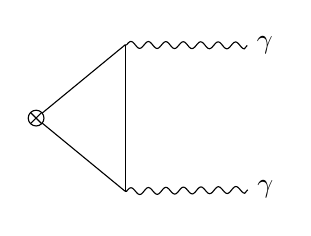
\begin{tikzpicture}
        \begin{feynman}
            \diagram [small, vertical=t3 to t2] {
            t1[crossed dot] -- t2 -- t3 -- t1,
            t2 -- [photon] p2 [particle=\(\gamma\)],
            t3 -- [photon] p1 [particle=\(\gamma\)],
            p1 -- [opacity=0] p2,
            };
            \end{feynman}
    \end{tikzpicture}
    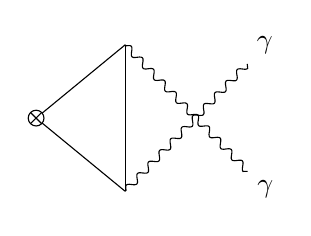
\begin{tikzpicture}
        \begin{feynman}
            \diagram [small, vertical=t3 to t2] {
            t1[crossed dot] -- t2 -- t3 -- t1,
            t2 -- [draw=none] p2 [particle=\(\gamma\)],
            t3 -- [draw=none] p1 [particle=\(\gamma\)],
            p1 -- [opacity=0] p2,
            };
            \diagram*{
                (t2)--[photon](p1),
                (t3)--[photon](p2),
            };
            \end{feynman}
    \end{tikzpicture}  
\end{equation*}


整体流和局部流的反常:

整体:会导致重要的物理后果,\textcolor{blue}{如,QCD中的$U(1)_A$反常能够推出$m_q\sim 1GeV$;$\pi^0\to\gamma\gamma$现象,QCD中的$U(1)_{PQ}$反常能够推出轴子的质量。}

局部:\textcolor{blue}{会破坏理论的可重整性。}

反常来自于路径积分中测度的变换:
\begin{align}
   \mD q \mD \bar{q} \stackrel{q\to e^{i\alpha \gamma_5 q}}{\longrightarrow} \mD q\mD \bar{q} e^{-i\int \md^4x[\frac{e^2}{16\pi^2F\tilde{F}}]}.
\end{align}
一个整体流反常有如下公式:
\begin{align}
   \partial_{\mu}j^{\mu,a}=\frac{g^2}{32\pi^2}{\rm Tr}[T^a\{t^b,t^c\}]\varepsilon^{\mu\nu\rho\sigma}F^b_{\mu\nu}F^c_{\rho\sigma}.
\end{align}

考虑$SU(3)$群,我们有轴矢流$j^{\mu}_5=\bar{q}\gamma^{\mu}\gamma_5 \mathbb{I} q$,其中$q^T=(u,d,s)$,因此
\begin{align}
   \begin{aligned}
      \partial_{\mu}j^{\mu}_5 =&\frac{g_s^2}{32\pi^2}{\rm Tr}[{\mathbb{I}}\{t^b,t^c\}]\varepsilon G^bG^c\\
      =&\frac{g_s^2}{32\pi^2}{\rm Tr}[{\mathbb{I}}]\cdot2{\rm Tr}[t^bt^c]\varepsilon G^bG^c\\
      =&\frac{g_s^2N_f}{32\pi^2}\varepsilon G^bG^b \to \textcolor{blue}{m_{\eta^{\prime}}\sim 1GeV.}
   \end{aligned}
\end{align}
其中的${\mathbb{I}}$是因为该诺特流与味空间无关。在最后一步,我们用了${\rm Tr}{\mathbb{I}}=N_f$,以及${\rm Tr}[t^bt^c]=\frac{1}{2}\delta^{bc}$。

考虑$U(1)_{EM}$群,我们有轴矢流$j_5^{\gamma,a}=\bar{q}\gamma^{\mu}\gamma_5T^aq$,以$a=3$为例,其中$Q={\rm diag}\{2/3,-1/3,-1/3\}$,
\begin{align}
   \begin{aligned}
      \partial_{\mu}j^{\mu,3}_5=&\frac{e^2}{32\pi^2}{\rm Tr}[T^3\{Q,Q\}]\varepsilon FF\\
      =&\frac{e^2}{32\pi^2}(\frac{N_C}{3})\varepsilon FF.
   \end{aligned}
\end{align}
\textcolor{blue}{在最后一步,我们用了$2{\rm Tr}[T^3 Q^2]=(\frac{N_C}{3})$}。
因此,积分测度变为
\begin{align}
   \mD q\mD\bar{q}\stackrel{q\to e^{i\alpha T^3\gamma_5}q}{\longrightarrow} \mD q\mD\bar{q}e^{-i\int \md^4x\alpha \frac{e^2}{32\pi^2}(\frac{N_C}{3})\varepsilon FF} ,
\end{align}
拉氏量变为
\begin{align}
   \mL \to \mL -\alpha \frac{e^2}{32\pi^2}(\frac{N_C}{3})\varepsilon FF.
\end{align}

考虑带有$\pi$介子的理论,假设系统沿着$T^3$方向进行$SU(3)_A$变换,可以证明$\pi^0\to\pi^0-\alpha f_{\pi}$。因此,为了保证$\mL_{\pi}$和$\mL_{QCD}$的变换方式一样,我们需要添加一项
\begin{align}
   \delta \mL_{\pi^0}=\frac{\pi^0}{f_{\pi}}\frac{e^2}{32\pi^2}\frac{N_C}{3}\varepsilon FF,
\end{align}
该项通常称为反常匹配,该项在$SU(3)_A$变化下为
\begin{align}
   \delta mL_{\pi^0}\to\delta mL_{\pi^0}\-\frac{\alpha f_{\pi}}{f_{\pi}}\frac{e^2}{32\pi^2}\frac{N_C}{3}\varepsilon FF,
\end{align}
刚好抵消了拉氏量的变化。而额外引入的$\delta\mL_{\pi^0}$项则会产生如下顶点:

%! TEX root = ../axions.tex
\begin{center}
    \feynmandiagram [medium, horizontal=a to b] {
    a[particle=$\pi^0$] --[scalar] b,
    b --[photon] t1[particle=$\gamma$],
    b --[photon] t2[particle=$\gamma$],
    };
\end{center}


由此,我们可以给出
\begin{align}
   \Gamma(\pi^0\to \gamma\gamma)=\frac{m_{\pi}^3\alpha^3}{64\pi^3f_{\pi}^2}(\frac{N_C}{3})\simeq 7.6eV (\frac{N_C}{3}),
\end{align}
而$\Gamma(\pi^0\to \gamma\gamma)_{\rm exp}\simeq 7.7eV$。





%! TEX root = ./axions.tex
\subsection{强CP问题}

首先考虑$U(1)$电磁规范理论,在不违反对称性的前提下,拉氏量可以写成
\begin{align*}
   \mathcal{L}\supset -F_{\mu\nu}F^{\mu\nu}+eA_{\mu}J^{\mu}+\theta F_{\mu\nu} F_{\lambda\sigma}\epsilon^{\mu\nu\lambda\sigma}
\end{align*}
而事实上,只有前两项出现在SM中,如果我们把$\theta$项展开可以得到$\vec{E}\cdot\vec{B}$,代入作用量中可以得到
\begin{align*}
   S=\int d^4 x\mathcal{L} \supset \int d^4x \theta \vec{E}\cdot\vec{B}
\end{align*}
将电场写作$\vec{E}=\nabla\Phi$,利用分部积分可以得到
\begin{align*}
   \int d^4x \vec{E}\cdot\vec{B}=\int d^4x\nabla\cdot(\Phi \vec{B})-\int d^4x \Phi \nabla\cdot\vec{B}
\end{align*}
其中第一项是表面项,如果没有磁单极子的存在,第二项等于0。表面项在经典物理中可以忽略。

先考虑表面项在量子力学中的作用,势能为谐振子势
\begin{align*}
   \mathcal{L}=\frac{\dot{x}^2}{2}-V(x)
\end{align*}
引入表面项后
\begin{align*}
   \mathcal{L}=\frac{\dot{x}^2}{2}-V(x)+\theta\dot{x}
\end{align*}
显然表面项不改变经典物理。如果我们计算考虑表面项后的哈密顿量,可以得到
\begin{align*}
   H=p\dot{x}-L=\frac{\dot{x}^2}{2}+V(x)
\end{align*}
哈密顿量不依赖于$\theta$,因此求解得到的波函数是一样的。

如果将势函数修改为周期谐振子势,即在$[-a,a]$是谐振子,然后不断平移,得到整体势函数。 周期谐振子势的求解要复杂得多,为此我们可以先计算$\langle x_f|e^{-HT}|x_i\rangle$在大$T$极限下,$|x\rangle$为位置本征态,
\begin{align*}
   \langle x_f|e^{-HT}|x_i\rangle=\sum_{n,m}\langle x_f|n\rangle\langle n|e^{-HT}|m\rangle \langle m |x_i\rangle=\sum_{n}\langle x_f|n\rangle\langle n|e^{-E_{n}T}|n\rangle \langle n |x_i\rangle
\end{align*}
在大$T$极限下,仅有基态占主导地位,因此$\langle x_f|e^{-HT}|x_i\rangle\simeq \langle x_f|0\rangle e^{-E_0T}\langle 0 |x_i\rangle$。

利用费曼路径积分的技巧,我们可以得到
\begin{align*}
   \langle x_f|e^{-HT}|x_i\rangle=N\int d \gamma e^{-S_{E}[\gamma]}
\end{align*}
其中$S_{E}$是欧式作用量($t\to \mbox{i}\tau$)
\begin{align*}
   S_{E}=\int d \tau (-(\frac{\dot{x}^2}{2}+V(x))+\mbox{i}\theta\dot{x})
\end{align*}
其中$\theta$项作为相位出现。我们知道在跃迁中起最大贡献的路径是使作用量取极小值的路径,而这正是经典路径。但在欧式作用量中,势变成了$-V$。因此问题变成了在$-V$中从$x_i$到$x_f$的跃迁。如果取$x_f=x_i$,则显然在一维谐振子中只有一条路径,即待着不动;而在周期谐振子势中,则可以有无穷多条路径,可以任意跨选择过峰,对于这些额外的路径我们称为瞬子。

\includegraphics[scale=0.35]{xiezhenzi.jpg}
 
这些不同的瞬子显然是不同的,有些可以是一个周期,有些可以是两个周期,我们称之为瞬子解的缠绕数。现在我们可以看出$\theta$项的意义了
\begin{align*}
   \int d\tau (\mbox{i}\theta x)\approx \mbox{i}\theta n
\end{align*}
其中$n$是缠绕数。因此$\theta$项是物理的,它告诉我们如何把这些瞬子加在一起。至于最终的答案以及细节计算可以参考Coleman的书,关键点在于$\theta$确实可以改变谱的结构。
\begin{align*}
   E=\frac{1}{2}\omega + 2Kcos\theta e^{-S_)}
\end{align*}.

考虑一个简单的无费米子的理论
\begin{align*}
   \mathcal{L}\supset -F_{\mu\nu}F^{\mu\nu}+\theta F_{\mu\nu}\tilde{F}^{\mu\nu}
\end{align*}
它的欧式路径积分为
\begin{align*}
   \int [d A]e^{-S_E[A]}
\end{align*}
同理,该积分主要由欧式空间运动方程的解给出。欧式运动方程由下面微分方程给出
\begin{align*}
   D_{\mu}F^{\mu\nu}=0
\end{align*}
为了求解方程,必须给定边界条件。如果有些解的能量是发散的,那么这些解对路径积分没有贡献。因此我们只需要找到那些有限能量的解,从而$F_{\mu\nu}$在无穷远处必须为0。但是$F_{\mu\nu}$为0,并不意味着$A$也为0。 This means, we seek boundary conditions where the potential is pure gauge out at infinity. 它在有限区域内具有非零场强,因此对欧式路径积分有贡献。如果时空是$R^4$的,那么它的边界就是$S^3$,那么我们其实就是在找一个从$S^3$到规范群$G$的映射。给定这样一个映射,如果可以连续变形到另外一个映射,那么就不用再单独计数,因为它也是路径积分的一部分。如果规范群是$U(1)$,那么所有从$S^3$映射到$U(1)$的群都可以连续变换到单位映射。因此仅有一个有限能量解,此时$\theta$项不重要。

可以发现,我们的映射是依赖时空维数的,如果是1+1维时空,那么边界就是$S^1$,从$S^1$到$U(1)$存在不平凡的映射。

同样,如果我们的规范群是$SU(N)$,也存在不平凡的映射。在$S^1$上,我们用缠绕数标记不同的映射。对于这些高维映射,我们用Pontryagin指标来标记。而对于这些解,我们都称之为瞬子。和缠绕数类似,这些指标告诉我们如何把不同的瞬子解加到一起。参考Coleman的书,可以给出$\theta$项的能量修正。因此$\theta$
是有物理意义的。
\begin{align*}
   E(\theta)\sim K cos\theta e^{-S_0}
\end{align*}
对于规范理论,可以证明瞬子的指数压低为$e^{-8\pi^2/g^2}$,其中$g$是规范耦合常数,对于$SU(2)$,耦合常数很小,因此几乎不讨论电弱的$\theta$项,但对于$SU(3)$,$\theta$项就不可以忽略了。


强相互作用的$SU(3)_C$是CP守恒的,但是低能情况下,一直存在一个问题:Weinberg的$U(1)_A$介子丢失问题。't Hooft的解决方案引发了人们对强CP问题的重新认识。

\subsubsection{$U(1)_A$介子丢失问题}


\newpage 

\renewcommand\refname{参考文献}

\bibliographystyle{unsrt}

\bibliography{axions}

\end{document}